\section{Outcome of Analysis}
\subsection{Initial Steps}
In order to perform analysis on the available data we used \verb|R studio|. After loading the datasets to a suitable dataframe format rigorous cleanup was performed since the data was not ideal for our scope of analysis. After we got the cleaned data for each analysis and/or step statistical analysis and shaping were performed so that it becomes easy to interface the data to its related tool such as \verb|plotly|, \verb|ggplot|. After feeding the shaped data to these tools we get human-readable visualizations that can be easily interpreted and inferred. Sections below are the observations we have found from our analysis.

\subsection{Proportion of Age}
Our first aim was to have an overall understanding of the mothers' age group and their proportions. After performing some statistical analysis we get two figures that show the trends of mothers of different age groups and their habits when it comes to having babies. In Figure: \ref{fig:age1} we can see that the age group of 15-19 and over 40 are the last 2 age groups that have babies while most mothers are from the age group of 30-34. 

\begin{figure}
  \centering
  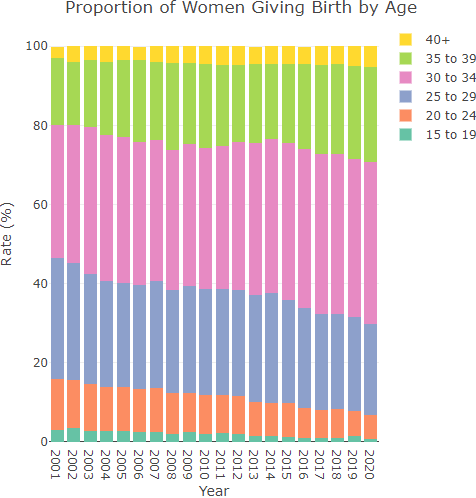
\includegraphics[width=0.35\textwidth]{img/age_group.png}
  \caption{Proportion of woman giving birth by age.}
  \label{fig:age1}
\end{figure}
\subsection{Trend Analysis of First Time Mothers}

\begin{figure}
  \centering
  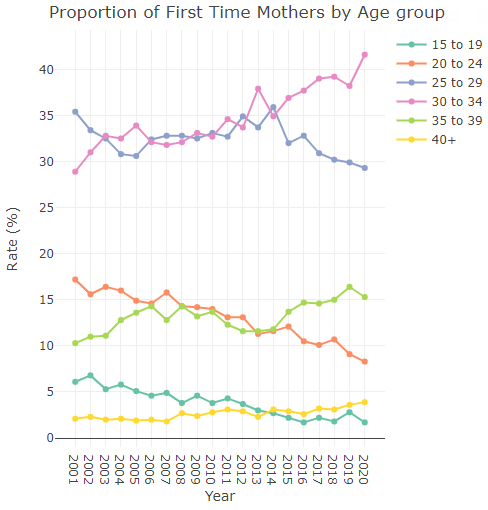
\includegraphics[width=0.35\textwidth]{img/first_time_age_group.png}
  \caption{Trends of first-time mother by age group.}
  \label{fig:age2}
\end{figure}
For a deeper understanding of what we have found in \verb|section 5.2| we were interested to see how many women became mothers for the first time. To achieve that we have generated Figure: \ref{fig:age2} where we can see that although mothers who are aged 40+ tend to have babies less the trend has been changing from the last decade and they have more birthrate than the age group of 15-19 years old. The low birthrate of 15-19 is understandably low as the legal age of consent is 16 except for Tasmania and South Australia which is 17 \cite{consentWebsite}.

Intuitively, this analysis leads us to ask how many women were becoming mothers for the first time each year so that we can observe a trend in women having babies. After generating figure: \ref{fig:firstTime} we can see that number of women becoming first-time mothers has increased over the years.


\begin{figure}
  \centering
  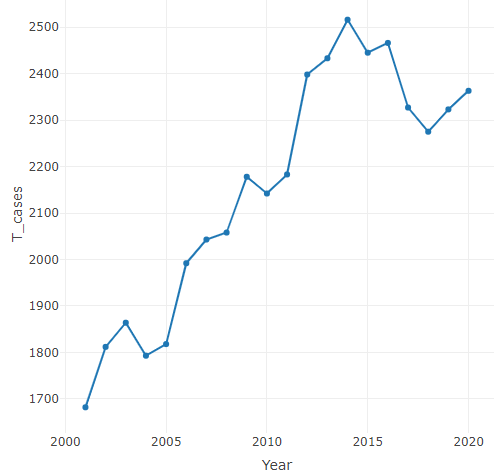
\includegraphics[width=0.35\textwidth]{img/first_time.png}
  \caption{Number of first-time mothers in each year.}
  \label{fig:firstTime}
\end{figure}